For the computational experiments a batch of tests was driven to find the best
parameters for the problem.
Afterwards two main tests was considered:
(a) using the well-known set of problems defined by Chu and Beasley \cite{Chu-Beasley-1998}
and (b) a large set of randomly generated instances using uniform distribution.

\subsection{The Chu-Beasley instances}

The set of MKP instances provided by Chu and Beasley was generated using a
procedure suggested by Freville and Plateau~\cite{freville1994efficient}, which
attempts to generate instances hard to solve.
The number of constraints $m$ varies among $5$, $10$ and $30$, and the number
of variables $n$ varies among $100$, $250$ and $500$.

The $w_{ij}$ were integer numbers drawn from the discrete uniform distribution
$U(0, 1000)$.
The capacity coefficient $c_i$ were set using
$b_i = \alpha\sum_{j=1}^{n} w_{ij}$ where $\alpha$ is a tightness ratio and
varies among $0.25$, $0.5$ and $0.75$.
For each combination of $(m,n,\alpha)$ parameters, $10$ random problems was generated,
totaling $270$ problems.
The profit $p_j$ of the items were correlated to $w_{ij}$ and generated as follows:
\begin{displaymath}
  p_j = \sum_{i=1}^m \frac{w_{ij}}{m} + 500q_j \qquad j = 1, \ldots, n
\end{displaymath}

\subsection{The set of random instances}

The second set of instances is composed by problems generated using a similar
setup.
The only differences is that the profit $p_j$ is also drawn from a discrete uniform
distribution $U(0, 1000)$.
For each combination of $(m, n, \alpha)$ parameter, $600$ random problems was
generated, totaling $16200$ problems.

\subsection{Experimental results}

All the experiments was run on a Intel$^R$ Core i5-3570 CPU @3.40GHz computer
with 4GB of RAM.
The SCE algorithm for MKP was implemented in C programming language.
For the set of random instance all best known solution was found by the solver
SCIP 3.0.1 running for at least 10 minutes.

After a previous test batch parameters for SCE was defined as shown in
Table~\ref{tab:params} and used in all executions of SCE.
\begin{table}
  \centering
  \begin{tabular}{c|c|l}
  \hline
  \multicolumn{1}{c}{\rule{0pt}{12pt} \bf Parameter \spc } & \multicolumn{1}{|c|}{\bf \spc Value \spc } & \multicolumn{1}{c}{\bf Description} \\[2pt]
  \hline\rule{0pt}{12pt}
  $N$  & $20$  & \spc \# of complexes \\
  $M$  & $20$  & \spc \# of individuals in each complex \\
  $P$  & $5$   & \spc \# of individuals in each subcomplex \\
  $K$  & $300$ & \spc \# of algorithm iterations \\
  $K'$ & $20$  & \spc \# of iterations used in the complex evolving process \\
  $c$  & $n/5$ & \spc \# of genes carried from parent in crossing process \\[2pt]
  \hline
  \end{tabular}
  \caption{Parameters used in SCE algorithm.}
  \label{tab:params}
\end{table}

Table~\ref{tab:chu} shows the performance of the SCE on the Chu-Beasley set of instance.
Each instance in the set was executed 10 times on SCE.
The \textit{SCE t} column shows the average execution time of SCE algorithm.
The \textit{gap} column shows the average ratio of the solution found by SCE and
the best known solution of each instance.
It can be observed that the SCE has a fast convergence speed, achieving high
quality solutions in few seconds.

\begin{table}
\parbox{.45\linewidth}{
\centering
{
  \renewcommand{\arraystretch}{1.5}%
\fontsize{8.5pt}{1em}\selectfont 
\begin{center}
\begin{tabular}{|r|r|r|rr|} \hline
\textbf{n}   & \textbf{m}  & \textbf{$\alpha$} & \textbf{SCE t (s)} & \textbf{gap (\%)} \\ \hline
100 & 5 & 0.25 & 0.79 & 96.5 \\
    &   & 0.5 & 0.81 & 97.4 \\
    &   & 0.75 & 0.83 & 98.9 \\ \cline{2-5}
    & 10 & 0.25 & 0.75 & 95.7 \\
    &    & 0.5 & 0.93 & 96.7 \\
    &    & 0.75 & 0.89 & 98.5 \\ \cline{2-5}
    & 30 & 0.25 & 1.01 & 95.4 \\
    &    & 0.5 & 1.07 & 96.4 \\
    &    & 0.75 & 0.99 & 98.2 \\ \cline{2-5}
    & \multicolumn{3}{r}{\textbf{average gap}}  & $\bf 97.1$  \\ \hline \hline
\textbf{n}   & \textbf{m}  & \textbf{$\alpha$} & \textbf{SCE t (s)} & \textbf{gap (\%)} \\ \hline
250 & 5 & 0.25 & 1.72 & 93.2 \\
    &   & 0.5 & 1.75 & 94.9 \\
    &   & 0.75 & 1.78 & 97.6 \\ \cline{2-5}
    & 10 & 0.25 & 1.84 & 93.1 \\
    &    & 0.5 & 1.84 & 94.6 \\
    &    & 0.75 & 1.81 & 97.2 \\ \cline{2-5}
    & 30 & 0.25 & 2.21 & 93.2 \\
    &    & 0.5 & 2.21 & 94.2 \\
    &    & 0.75 & 2.31 & 96.6 \\ \cline{2-5}
    & \multicolumn{3}{r}{\textbf{average gap}}  & $\bf 95.0$  \\ \hline \hline
\textbf{n}   & \textbf{m}  & \textbf{$\alpha$} & \textbf{SCE t (s)} & \textbf{gap (\%)} \\ \hline
500 & 5 & 0.25 & 3.16 & 91.4 \\
    &   & 0.5 & 3.18 & 93.4 \\
    &   & 0.75 & 3.34 & 96.4 \\ \cline{2-5}
    & 10 & 0.25 & 3.39 & 91.7 \\
    &    & 0.5 & 3.37 & 93.1 \\
    &    & 0.75 & 3.44 & 96.2 \\ \cline{2-5}
    & 30 & 0.25 & 3.83 & 91.4 \\
    &    & 0.5 & 3.90 & 92.6 \\
    &    & 0.75 & 3.99 & 96.0 \\ \cline{2-5}
    & \multicolumn{3}{r}{\textbf{average gap}}  & $\bf 93.6$  \\ \hline
\end{tabular}
\end{center}

}
 \caption{SCE performance on Chu-Beasley problems.}
 \label{tab:chu}
}
\hfill
\parbox{.45\linewidth}{
\centering
{
  \begin{tabular}[c]{|r|r|r|rrr|} \hline
\textbf{n}   & \textbf{m}  & \textbf{$\alpha$}    &\textbf{SCIP t (s)}& \textbf{SCE t (s)} & \textbf{gap (\%)} \\ \hline
$500$ & $10$ & $0.25$ & $278.85$ & $  2.23$  & $96.1$ \\
    &    & $0.50$ & $177.32$ & $  2.14$  & $98.4$ \\
    &    & $0.75$ & $  8.47$ & $  1.87$  & $99.6$ \\ \cline{2-6}
	   & \multicolumn{4}{r}{\textbf{average gap}}  & $\bf 98.0$  \\ \cline{2-6}
    & $20$ & $0.25$ & $284.11$ & $  2.30$  & $96.7$ \\
    &    & $0.50$ & $275.68$ & $  2.16$  & $98.6$ \\
    &    & $0.75$ & $ 33.67$ & $  1.90$  & $99.7$ \\ \cline{2-6}
	   & \multicolumn{4}{r}{\textbf{average gap}}  & $\bf 98.3$  \\ \cline{2-6}
    & $30$ & $0.25$ & $283.78$ & $  2.50$  & $96.9$ \\
    &    & $0.50$ & $283.54$ & $  2.32$  & $98.7$ \\
    &    & $0.75$ & $ 71.66$ & $  1.96$  & $99.7$ \\ \cline{2-6}
    & \multicolumn{4}{r}{\textbf{average gap}}  & $\bf 98.3$  \\ \hline
\end{tabular}
%Chu-Beasley problems.

}
 \caption{SCE performance on the random generated problems.}
 \label{tab:rand}
}
\end{table}

\begin{figure}
  \centering
  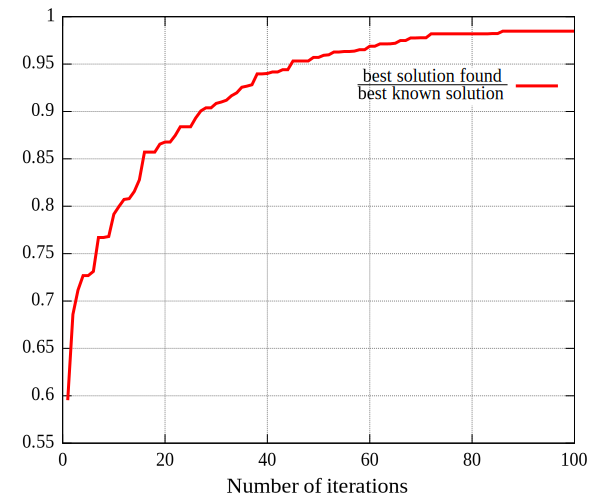
\includegraphics[scale=0.5]{imgs/iter}
  \caption{Convergence process of SCE for MKP
    for a problem with $n=500$, $m=30$ and $t=0.50$.}
  \label{fig:iter}
\end{figure}

The fast convergence speed of SCE for MKP can be noticed in Fig.~\ref{fig:iter}.
The figure shows for each iterations step, the quality of best solution found
for the first $100$ iterations.
The problem instance used was taken from the second set of problem (random instances).
The best known solution was found with $600$s of execution on SCIP solver and
the execution of the SCE algorithm expended $1.1$ seconds.
